
Da die exakte Berechnung einer Kollision zwischen zwei Objekten $o_0, o_1 \in \obj$ signifikant viel Rechenleistung benötigt //TODO (Test und referenz auf l2), ist eine Vorfilterung der möglichen Objektpaare sinnvoll, die die meisten Paare schon vorher ausschließt.\\
Zu diesem Zweck werden zu jedem Objekt Hüllkörper angegeben, die die Objekte durch die Eigenschaft $B_o \supseteq K_o$ abstrahieren, da gilt $K_{o0} \cap K_{o1} \Rightarrow B_{o0} \cap B_{o1}$, d.h.~ die Menge aller Paare mit exakter Kollision ist in jedem Fall in der Menge aller Paare enthalten $ \{ (o_0, o_1) | B_{o0} \cap B_{o1} \} \supseteq \{ (o_0, o_1) | K_{o0} \cap K_{o1} \} $.
Die weiteren Eigenschaften der Hüllkörper sollen den Filterungsprozess erheblich vereinfachen, da Kollisionen unter diesen u.U. leichter zu errechnen sind. Hier wird als Hüllkörper eine AABB verwendet, deren hier praktische Eigenschaften in Abschnitt \ref{sec:AABB} beschrieben sind.\\
Im Kontext des gesamten Abschnitts \ref{sec:l1} wird als Abstraktionsgrad für ein Objekt solch eine AABB verwendet. Für bestimmte Zwecke, meist logische Kollisionen (vgl. \ref{sec:usages}), ist diese abstrakte Kollision sogar schon ausreichend, um eine Reaktion einzuleiten.\\
Um verschiedene Arten der Kollision behandeln zu können und die Objektpaare dem richtigen Algorithmus für die nächste Stufe zuführen zu können, wurde im Rahmen des Projekts eine Komponente erstellt, die dieses Problem mit austauschbarem Vorfilterungsalgorithmus löst. (Ungenügende Ansätze der Behandlung verschiedener Kollisionstypen unter Verwendung eines nicht austauschbaren Vorfilterungsalgorithmus haben schon vor dem Projektstart in der Codebasis existiert). \\
Logische und physikalische Kollisionen werden als (lokale) Interaktionen zusammengefasst und werden in 2 Kategorien eingeteilt:
\begin{enumerate}
\item Symmetrische Interaktionen:\\
Beide Objekte des Objektpaares gehören der selben Klasse an (z.B: die Kollision rigider Objekte, wie sie in Abschnitt~\ref{sec:l2} beschrieben wird).
\item Asymmetrische Interaktionen:\\
Objektpaare setzen sich aus 2 Objekten verschiedener Klassen zusammen (z.B. Projektil und treffbares Objekt). Kollisionen innerhalb der selben Klasse treten hier nicht auf (Projektile interagieren nicht mit anderen Projektilen).
\end{enumerate}

In jeder o.g. Kategorie können mehrere Interaktionstypen enthalten sein. Beispiele für 2 asymmetrische Interaktionstypen sind Interaktion von Projektil mit treffbarem Objekt oder Trigger-Bereich mit triggerndem Objekt. Jeder Typ wird hier einzeln betrachtet und ihm kann so ein eigener Vorfilterungsalgorithmus zugewiesen werden, der entsprechend zugeschnitten und problemspezifisch optimiert werden kann.
Die Aufgabe des Vorfilterungsalgorithmus unterscheidet sich je nach Kategorie der Interaktion etwas:
\begin{enumerate}
\item Symmetrische Interaktionen: Aus einer Menge von Objekten $\obj$ werden Objektpaare ausgewählt, deren AABBs sich überschneiden. Ein beliebiges der beiden Objekte muss dann über die Interaktion mit dem Partner informiert werden, d.h. die Objekte sind vertauschbar.
Als untere Schranke kann man $\Omega (|\obj|+|C|)$ angeben, wobei $|C|$ die Anzahl der tatsächlichen Überschneidungen ist. Die obere Schranke $\mathcal{O}(|\obj|^2)$ erhält man durch naives Ausprobieren jeder Kombination.
\item Asymmetrische Interaktionen: Es gibt 2 Mengen $\obj_M, \obj_S$,die Menge der Master-Objekte und die Menge der Slave-Objekte. Daraus werden alle Objektpaare mit jeweils einem Mitglied aus jeder Menge ausgewählt, genau dann, wenn deren AABBs sich überschneiden. Das Master-Objekt ist dabei der aktive Part, der vom Algorithmus bei einer Interaktion informiert wird. Die Zuweisung ist also zur Compilezeit festgelegt. Wenn also ein Filteralgorithmus 2 interne Mengen unterschiedlich behandelt, aber die Zuweisung dieser 2 Mengen an Master/Slave-Menge beliebig sein soll, muss dieser diese Flexibilität selbst extra implementieren. Als untere Schranke kann man $\Omega(|\obj_M|+|\obj_S|+|C|)$ angeben. Die obere Schranke $\mathcal{O}(|\obj_M|+|\obj_S|)$ erhält man durch naives Ausprobieren jeder Kombination.
\end{enumerate}

Für die Laufzeit bei praktischen Problemen sei angemerkt, dass die Konstante oft eben so wichtig zu betrachten ist wie die asymptotische Komplexität (z.B. siehe Abb.~\ref{fig:symmetricComparison} C)\\
Im Folgenden werden 2 Algorithmen, die im Rahmen des Projekts implementiert werden, näher beschrieben.


\subsection{Box Sort}
\label{sec:boxsort}
Bei Box-Sort \cite{houthuys1987box}
%GRR citation wrongly displayed, seemingly not in bibliography either??????????????????????????????
 wird eine binäre Baumstruktur aufgebaut, in der anschließend nach einem Raumbereich (einer AABB, der Query-Box
\newcommand{\qb}{\operatorname{QB}}
 $\qb$) gesucht werden kann, sodass alle damit überlappenden einsortierten AABBs gefunden werden. Aufgrund der Mehrdimensionalität und dem Einsortieren von Bereichen statt Punkten müssen Anpassungen der Baum-Datenstruktur vorgenommen werden.\\
Ein Knoten referenziert genau eine einsortierte AABB. Als Sortierschlüssel wird dort das untere Extremum der einsortierten AABB in einer bestimmten Dimension, $x_{min},y_{min}$ oder $z_{min}$  (Definition vgl. \ref{sec:aabb}) gewählt, es gilt also $\operatorname{key} \in BB_{min}, \operatorname{key} \in \mathcal{S} $. 
Ist das obere Extremum der Query-Box in dieser Dimension kleiner als der Schlüssel, kann die Baumhälfte, die höhere Werte beinhaltet, ausgeschlossen werden und muss nicht mehr durchsucht werden. \\
Die Sortierdimension ist hier für jeden Knoten individuell wählbar.\\
Um die untere Baumhälfte ausschließen zu können, müssen jedoch eine weitere Information vorliegen: Die maximale Ausdehnung der AABBs im unteren Teilbaum nach oben (in der vorher festgelegten Sortierdimension). Der Knoten kann diese jedoch nicht festlegen, da die Sortierung nur anhand der unteren Extrema erfolgt. Deshalb muss jeder Knoten, der darunter liegt, berücksichtigt werden und der Maximalwert aller ermittelt werden. Dies geschieht beim Baumaufbau und wird danach im Knoten vermerkt.\\
Wird zu beiden Teilbäumen auch der jeweils andere Extremwert gespeichert, entsteht eine eindimensionale AABB und beide Teilbäume können identisch behandelt werden. Dann kann für jeden Teilbaum individuell ein Überlappungstest bestimmen, ob sich $\qb$ mit dem Teilbaum überschneidet. So können unter bestimmten Umständen sogar beide Teilbäume ausgeschlossen werden. Ein Beispiel dafür sieht man in Abb.~\ref{fig:boxsortNode}.\\

\begin{figure}
    \centering
    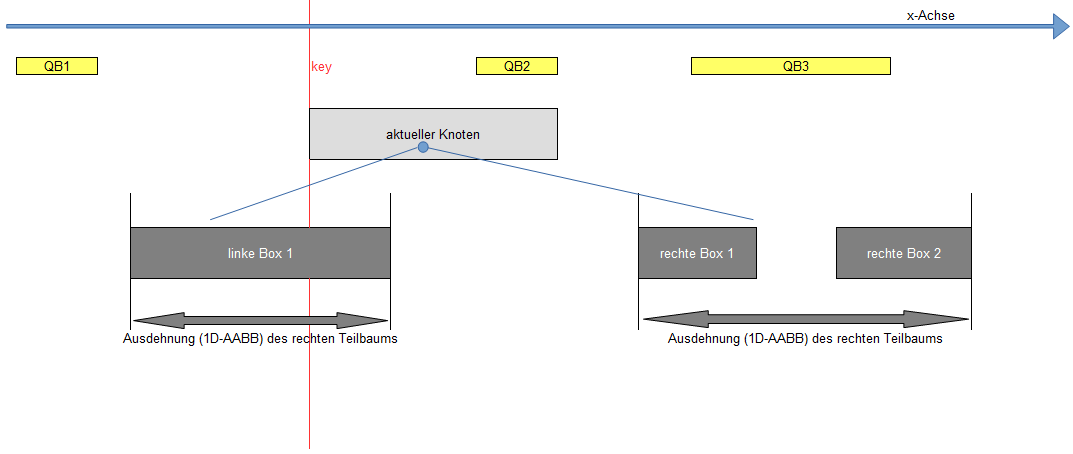
\includegraphics[width=1.0\textwidth]{./res/BoxsortNode.png}
    \caption{2D-Beispiel für einen Knoten (mittig, hellgrau) im Suchbaum bei Box-Sort. x-Achse zur Sortierung. Teilbäume nur durch darin enthaltene AABB(unten, dunkelgrau) dargestellt, Query Boxes (oben, gelb).}
    \label{fig:boxsortNode}
\end{figure}

Man sieht in Abb.~\ref{fig:boxsortNode}, dass QB1 sich komplett links der Bereiche der beiden Teilbäume befindet. Der Suchlauf endet für QB1 somit direkt bei dem dargestellten aktuellen Knoten. Ebenso bei QB2, die sich mit keinem Bereich der Teilbäume überschneidet, sie befindet sich diesmal aber zwischen beiden. Solch eine Lage muss im Allgemeinen nicht zwangsläufig existieren, denn die Bereiche der beiden Teilbäume können auch überlappen. QB3 hingegen überlappt mit dem rechten Teilbaum. Für die Suche scheidet in diesem Fall also nur der linke Teilbaum aus. Diese wird im rechten Teilbaum rekursiv fortgesetzt. Man kann auch Query-Boxes konstruieren, sodass eine Überlappung mit beiden Teilbäumen auftritt. Dann muss die Suche in beiden rekursiv fortgesetzt werden.\\

Der eigentliche Sortiervorgang zum Aufbau des Baums wird mit einer Variante von Quicksort durchgeführt. Dabei wird das Pivot-Element zum Knoten und die restlichen Elemente werden entsprechend des Schlüssels in die beiden Teilbäumen aufgeteilt. Bei der Zuteilung wird nebenbei die 1D-AABB des Teilbaums ermittelt, indem die Ausdehnung bei jedem Zuteilungsschritt ggf. vergrößert wird, um das aktuelle Element zu berücksichtigen.\\
Als Heuristik für das Finden des Pivot-Elements wird der Median einer zufälligen Auswahl von bis zu 9 Elementen gewählt. Dies ist ein einfacher Kompromiss zwischen rechenaufwändigeren Verfahren, die genauer wären und der zufälligen Wahl des Pivot-Elements, die aber einen weniger idealen, tieferen Baum liefert, dessen Durchlauf deshalb länger dauern würde. Die Sortierdimension wird an der Wurzel des gesamten Binärbaums auf die x-Achse festgelegt. 
Beim Einsortieren in die beiden Teilbäume wird eine Heuristik berechnet, die im jeweiligen Teilbaum die beste Sortierdimension abschätzt. Dafür wird für jede Dimension die durchschnittliche Größe der Objekte im Teilbaum in dieser Dimension berechnet. Damit kann man die Dichte der Objekte in jeder Dimension abschätzen, wenn man den Gesamtbereich kennt, den die AABBs einnehmen. Gewählt wird die Dimension niedrigster Dichte.\\
Es müssen für den Box Sort-Algorithmus vor dem Start erst alle Objekte gesammelt werden. Im asymmetrischen Fall muss dann entschieden werden, aus welcher Menge ($\obj_M$ oder $\obj_S$) der Baum aufgebaut wird. Die Menge der Objekte für den Baumaufbau sei $\obj_T$. Die Elemente der anderen Menge ($\obj_Q$) werden dann nacheinander als QB gesucht. Der Benutzer kann Einfluss auf die Zuteilung nehmen. Die Basis der dann automatisch getroffenen Wahl ist ein Vergleich der Anzahl von Elementen je Klasse. Der Grund dafür wird deutlich, wenn die Laufzeit im erwarteten Fall betrachtet wird: $\mathcal{O}(|\obj_T|*log(|\obj_T|))$ für den Baumaufbau (folgt aus Quicksort). Wenn eine ausreichende Verteilung im Raum vorliegt und die Größe von QB in der selben Größenordnung ist wie Elemente aus $\obj_T$, dann benötigt die Suche $\mathcal{O}(log(|\obj_T|))$ Zeit \cite{houthuys1987box}. Insgesamt wird also für das Finden aller Überlappungen $\mathcal{O}(|\obj_T|*log(|\obj_T|)+|\obj_Q|*log(|\obj_T|))$ Zeit benötigt. Anhand dieser Form steht die Vermutung nahe, dass die Wahl von $\obj_T$ immer auf die kleinere Menge fallen sollte. In der Praxis ist vor den Termen $|\obj_T|*log(|\obj_T|)$ und $|\obj_Q|*log(|\obj_T|)$ aber ein jeweils anderer Vorfaktor, der deshalb auch beachtet werden muss. Messungen ergaben einen nahezu konstanten Vorfaktor beim Baumaufbau. Für den Abfrage-Durchlauf  ist der Faktor jedoch stark abhängig von der konkreten Verteilung der eingegebenen AABBs. Messungen ergeben einen um den Faktor von ca.~3 geringeren Vorfaktor unter stark idealisierten Bedingungen, einen nahezu identischen unter moderaten Bedingungen und einen ca. 3-mal größeren unter erschwerten Bedingungen (Durchschnittliche Kollisionen pro Objekt>3). Den Benchmark-Ergebnissen in ~\ref{sec:benchmark} kann man entnehmen, dass wenn die beiden Mengen die gleiche Verteilung aufweisen die kleinere Menge meist die bessere Wahl ist, vor allem bei geringer Dichte der Objektverteilung. Um trotzdem offen für zukünftige problemspezifische Erkenntnisse zu sein, bleibt die Option, die größere oder die kleinere Menge zu wählen. Dazu kann ein Präferenz-Faktor angegeben werden, der vor der Entscheidung mit der Anzahl der Master-Elemente multipliziert wird. Mit Extremwerten kann der Benutzer einstellen, dass nur eine der beiden Mengen für den Baum verwendet werden darf. Dies wird für Fälle gebraucht, wo die o.g. Bedingungen für die Komplexität der Suche im Baum nur für eine der beiden Mengen zutreffen.\\
 
 
Im symmetrischen Fall wird jedes Objekt sowohl in den Baum einsortiert als auch als QB in dem Baum gesucht. Dabei muss das Ergebnis des Paares $(qb, qb) : qb\in\{AABB_o | o \in \obj\}$ aus den Ergebnissen nachträglich wieder entfernt werden. Außerdem muss dafür gesorgt werden, dass bei einem interagierenden Objektpaar nur ein Aufruf erfolgt, obwohl beide Richtungen als Suchergebnis gefunden werden.\\

\subsection{Spatial Hashing}
\label{sec:spatialHashing}
Die Grundidee besteht hier dabei, den Raum in viele Bereiche (sog. Chunks) aufzuteilen und Kollisionspaare nur innerhalb dieser Teilbereiche zu suchen. Sind 2 Objekte weit voneinander entfernt und somit nicht im selben Chunk, ist eine Überschneidung der AABBs nicht möglich und muss deshalb auch nicht betrachtet werden. Wegen der Einfachheit bietet es sich an, regelmäßige Interavalle, durch achsenparallele Linien bzw. Ebenen getrennt zu verwenden, meist mit identischer Größe in jeder Dimension. Ein Beispiel für 2 Dimensionen sieht man in Abb.~\ref{fig:spatialHashing}.

\begin{figure}
    \centering
    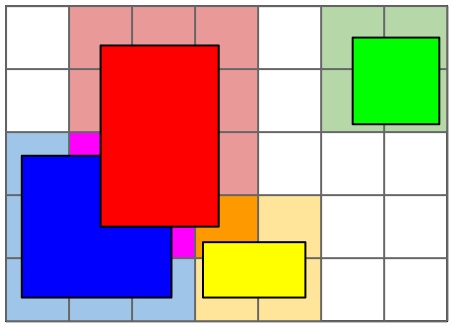
\includegraphics[width=0.5\textwidth]{./res/spatialHashingAABB.png}
    \caption{2D-Beispiel von Spatial Hashing von AABBs (stark gefärbte Rechtecke). Die leicht gefärbten Bereiche sind Chunks, die ein Objekt der entsprechenden Farbe(n) beinhalten. Bildquelle: \cite{spatialHashing}}
    \label{fig:spatialHashing}
\end{figure}

Man sieht in Abb.~\ref{fig:spatialHashing}, dass Objekte mit mehreren Chunks überlappen können. Ein Objekt muss sich in jedem Chunk anmelden, das sich mit seiner AABB überschneidet, zu sehen z.B. beim grünen Objekt, das sich in den 4 Chunks rechts oben anmelden muss. Gibt es keine weiteren Objekte in den Chunks, wo sich das Objekt angemeldet hat, müssen keine potentiellen Kollisionen berechnet werden.\\

Im symmetrischen Fall, wenn dies für alle Objekte der Fall ist, ist die optimale Komplexität $\mathcal{O}(|\obj|)$  bei konstanter Maximalgröße von Objekten erreicht.\\
Im asymmetrischen Fall können mehrere Objekte im selben Chunk angemeldet sein, ohne dass eine Kollision auftreten muss, solange die Objekte alle vom selben Typ sind. Ist diese Bedingung für alle Chunks wahr ist die optimale Komplexität von $\mathcal{O}(|\obj_M|+|\obj_S|)$ bei konstanter Maximalgröße von Objekten erreicht. \\
Werden mehrere Objekte, die für eine Kollision kompatibel sind, in einem Chunk angemeldet, so müssen alle potentiellen Kollisionspaare überprüft werden (hier mit naivem $\mathcal{O}(|\obj|^2)$ bzw. $\mathcal{O}(|\obj_M|*|\obj_S|)$ Algorithmus). Die Überprüfung kann entweder direkt bei der Anmeldung erfolgen (hier implementiert) oder erst nach Eintragung aller Objekte erfolgen.\\
Ein potentielles Problem kann in Abb.~\ref{fig:spatialHashing} bei der Überschneidung des roten und blauen Objekts betrachtet werden. Erfolgt eine Überlappung in mehreren Chunks, besteht die Gefahr der mehrfachen Behandlung von Kollisionen. Deshalb wird während der Partnerfindung ein Hashtable mit schon behandelten Objekten mitgeführt, womit effizient Duplikate vermieden werden. Auf diese Maßnahme kann verzichtet werden, wenn sich das Objekt nur in einem Chunk befindet.\\
Aus Einfachheitsgründen wurde als Chunk genau eine kubische Einheit (Seitenlänge 1) im System $\mathcal{S}^3$ gewählt. Ein Chunk lässt sich also eindeutig durch Koordinaten aus $\mathcal{I}^3$ identifizieren. Um das Anlegen vieler leerer Chunks zu vermeiden und trotzdem schnellen Zugriff zu haben, wird ein Hashtable zur Verwaltung der Chunks verwendet. Dazu wurde eine passende Hashfunktion gesucht und eingebunden, die plattformunabhängig aber dennoch mit sehr geringer Laufzeit $HASH: \mathcal{I}^3 \mapsto \mathcal{I}_{64}$ mit $\mathcal{I}_{64}$ als 64-Bit Integer einem Hashwert zuordnet.\\
Der Idealfall an dem Spatial-Hashing asymptotisch optimal wird wurde bereits beschrieben. In der Praxis tritt dies jedoch nur selten auf. Problematisch können dort z.B. große Objekte werden, denn die Anzahl Chunks, wo eine Anmeldung erforderlich ist (und damit auch die Laufzeit) steigt dann linear mit dem Volumen. Ein weiterer Problemfall ist, wenn zu viele Objekte in einem Chunk sind. Denn selbst wenn sie sich nicht überschneiden, ist dann eine $\mathcal{O}(|\obj|^2)$ bzw. $\mathcal{O}(|\obj_M|*|\obj_S|)$ Auflösung erforderlich ($\obj, \obj_M, \obj_S$ hier Mengen von Objekten im Chunk). Ob dieser Algorithmus für den Einsatz sinnvoll ist, hängt also davon ab, ob diese Probleme bei dem bestimmten Interaktionstyp auftreten, wo er eingesetzt werden soll.\\


\subsection{Benchmark und Vergleich der Verfahren}
\label{sec:benchmark}
Um die Performanz der Algorithmen bei verschiedenen Szenarien objektiv bewerten zu können, wurde im Rahmen des Projektes eine Benchmark-Umgebung implementiert. Getestet wurden verschiedene Szenarien und deren Parameter. Gemeinsam haben alle Szenarien die Testparameter Problemgröße (gesamte Objektanzahl) und absolute Größe der Objekte (aus $\mathcal{S}$, hier der durchschnittliche Wert für die Größe in der Dimension, wo das Objekt am größten ist).\\

Das Standardszenario ist eine Gleichverteilung von Objekten im Raum. 
Ein zusätzlicher Testparameter hier ist die Dichte der Objekte, welche das Verhältnis der absoluten Größe zur Durchschnittsdistanz der Mittelpunkte darstellt. Die asymmetrische Variante hat zusätzlich noch das Verhältnis der Menge an Objekten beider Klassen als Testparameter. Die Größe des Erzeugungsbereichs ist bei beiden Klassen identisch. Die Objektanzahl bezieht sich bei allen asymmetrischen Szenarien auf die Gesamtzahl der Objekte (also $|\obj_M| + |\obj_S|$)\\
Ein weiteres rein asymmetrisches Szenario \glqq Shotgun\grqq ~modelliert eine Menge an Projektilen und Zielen. Die Ziele sind weiterhin gleichverteilt, die Projektile modellieren jedoch eine Schrotladung, bei der viele Projektile relativ nahe zusammen in eine sehr ähnliche Richtung fliegen. Dies bedeutet, dass die AABBs der Projektile sich weitgehend überlappen (AABBs werden über den gesamten Raum ausgedehnt, durch den sich Objekte im Laufe eines Ticks bewegen, siehe \ref{sec:bounding_volume}). Sie werden aber alle nur in einem Teilbereich erzeugt, der nicht dem gesamten Erzeugungsbereich der Zielobjekte entspricht. Ein Testparameter beschreibt die erwartete Anzahl Ziele im Erzeugungsbereich der Projektile. Das Verhältnis zwischen der Menge der Zielobjekte und der Projektile ist ein weiterer Parameter.\\
Die Benchmark-Umgebung setzt den Seed des verwendeten Zufallsgenerators abhängig von den Parametern eines Szenarios, aber nicht abhängig vom verwendeten Algorithmus. So müssen verschiedene Algorithmen die exakt selbe Problemstellung lösen. Um Messstörungen herauszufiltern, wird jedes Experiment einige Male wiederholt und der Median für die weitere Untersuchung verwendet. Eines dieser Ergebnisse wird im Folgenden als Sample bezeichnet. Um die Probemenge zu erhöhen wurde ein Dummy-Parameter (mit 4 möglichen Werten) eingefügt, der den Seed ändert aber sonst keine Auswirkungen hat. Dies führt dazu, dass 4 Samples zu jeder Kombination von wirksamen Parametern existieren.\\
%//TODO alle Absätze überprüfen
Für die im Folgenden gezeigten Daten wurden alle Benchmarks auf einem PC mit Intel i7-4790K CPU bei 4,5GHz mit 2400MHz Dual-Channel RAM ausgeführt und die Daten in einer Datei gespeichert. Diese wird von Python-Code eingelesen, der zur Auswertung der Benchmark-Daten geschrieben wurde. Dort werden mit Hilfe von Matplotlib, einer Programmbibliothek, Diagramme zu den Daten erzeugt, die im Folgenden ausgewertet werden.\\
Zunächst soll bei Box Sort die Wahl der Objektmenge ($\obj_M$ oder $\obj_S$) für den Baum untersucht werden (in Abschnitt~\ref{sec:boxsort} theoretisch betrachtetes Problem). Zu diesem Zweck wird das Verhältnis der Ausführungszeiten beider Möglichkeiten betrachtet. Ist es größer als 1, bedeutet dies hier, dass es mehr Ausführungszeit benötigt hat, die Master-Klasse für den Baum zu verwenden, d.h. die Slave-Klasse ist dann die bessere Wahl für den Baum.\\

\begin{figure}
    \centering
    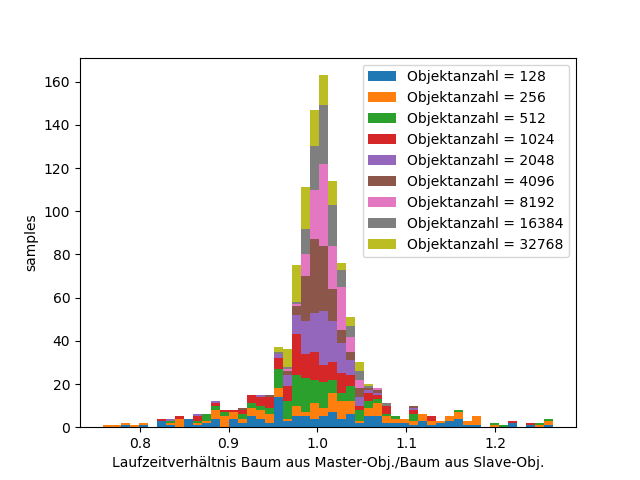
\includegraphics[width=1.0\textwidth]{./res/boxsortChoice-reference.png}
    \caption{Einfluss der Wahl der Objektmenge für den Baumaufbau beim Box Sort, wenn 2 gleich große Mengen getestet wurden, die beide statistisch gleichverteilt über den selben Raum sind (Referenzfall).  Dargestellt ist ein Histogramm mit nach Objektzahl getrennten Samples, mit den jeweiligen Balken aufeinandergestapelt.}
    \label{fig:boxsortCoice-reference}
\end{figure}

Als Referenz soll zunächst die Wahl bei einer Gleichverteilung betrachtet werden, zunächst mit einer identischen Menge an Objekten beider Klassen. Abb.~\ref{fig:boxsortCoice-reference} zeigt, dass in diesem Referenzfall kein signifikanter Unterschied zwischen beiden besteht und die sichtbaren Unterschiede wahrscheinlich vom Zufall stammen. Zu sehen ist, dass die stärkeren Abweichungen im Randbereich häufiger bei niedrigen Objektzahlen und damit auch niedrigen absoluten Laufzeiten auftreten.\\


\begin{figure*}
	\begin{subfigure}[t]{0.50\textwidth}
		\centering
		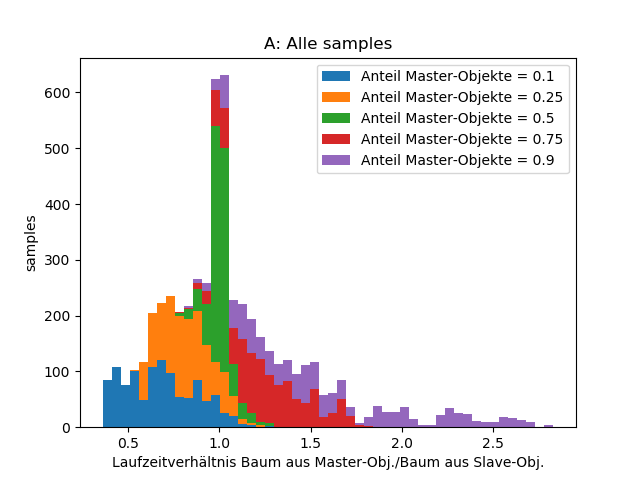
\includegraphics[width=1\textwidth]{./res/boxsortChoice-uniform-A.png}
		
		\label{fig:boxsortChoice-uniform-A}
	\end{subfigure}
\hfill
	\begin{subfigure}[t]{0.50\textwidth}
		\centering
		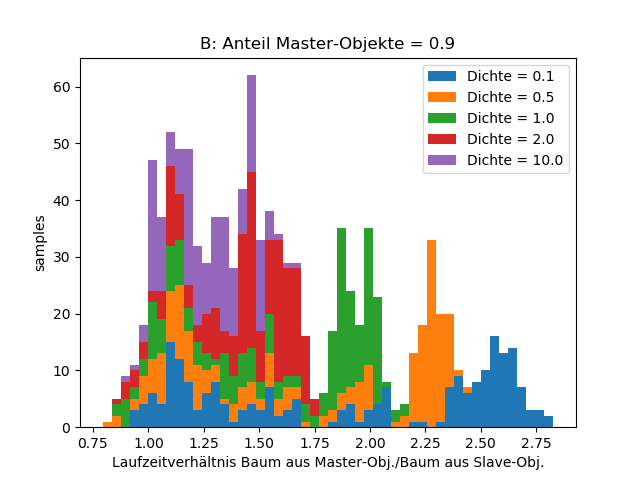
\includegraphics[width=1\textwidth]{./res/boxsortChoice-uniform-B.png}

		\label{fig:boxsortChoice-uniform-B}
	\end{subfigure}
\vskip\baselineskip
	\begin{subfigure}[t]{0.50\textwidth}
		\centering
		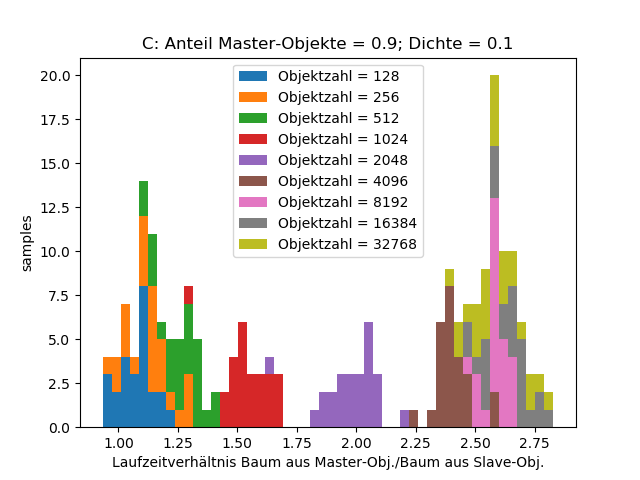
\includegraphics[width=1\textwidth]{./res/boxsortChoice-uniform-C.png}

		\label{fig:boxsortChoice-uniform-C}
	\end{subfigure}
\hfill
	\begin{subfigure}[t]{0.50\textwidth}
		\centering
		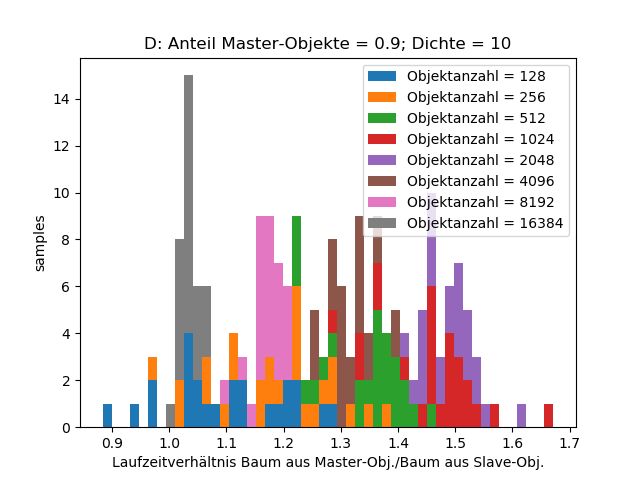
\includegraphics[width=1\textwidth]{./res/boxsortChoice-uniform-D.png}

		\label{fig:boxsortChoice-uniform-D}
	\end{subfigure}

	\caption{Untersuchung der Auswirkungen verschiedener Parameter auf das Verhältnis der Laufzeiten des Box Sort Algorithmus im gleichverteilten Szenario. Dargestellt sind Histogramme mit nach einem Parameter getrennten Samples, mit den jeweiligen Balken aufeinandergestapelt.}
	\label{fig:boxsortChoice-uniform}
\end{figure*}


Wenn die Objektzahl je Klasse nicht mehr identisch ist, können die Vermutungen zur Klassenwahl aus Abschnitt~\ref{sec:boxsort} untersucht werden. Mehrere Untersuchungen dazu werden in Abb.~\ref{fig:boxsortChoice-uniform} gezeigt. Abb.~\ref{fig:boxsortChoice-uniform} A zeigt alle Samples. Zu erkennen ist, dass bei den getesteten Parametern der Baum aus der kleineren Menge gebildet werden sollte. Um genauer zu betrachten, welche Parameterkombination zu welchem Unterschied führt, werden zunächst in Abb.~\ref{fig:boxsortChoice-uniform} B die Samples auf diejenigen beschränkt, wo der Anteil Master-Objekte 90\% beträgt. Erkennbar ist, dass der Wertebereich stark von der Dichte abhängig ist, wobei die geringste Dichte die höchste Streuung aufweist. Um dies weiter zu untersuchen, zeigt Abb.~\ref{fig:boxsortChoice-uniform} C davon nur die geringste getestete Dichte. Zu sehen ist dort, dass die Unterschiede bei weniger Objekten gegen 0\% gehen, bei vielen Objekten gegen etwa +150\%. Die Beobachtung bei vielen Objekten passt zu den in Abschnitt~\ref{sec:boxsort} beobachteten Vorfaktoren, was auch bei vielen Objekten erfolgte. Für den Fall höherer Dichte scheinen die dort ermittelten Werte nicht mit den im Benchmark gemessenen Werten übereinzustimmen, die in Abb.~\ref{fig:boxsortChoice-uniform} D zu sehen sind. Dies weist auf einen weiteren versteckten Faktor hin. Man könnte weitere Tests für höhere Dichten durchführen, dort ist Box-Sort jedoch keine sinnvolle Wahl mehr, da für praktische Objektzahlen dann selbst der naive Algorithmus noch schneller wäre. Dort wäre außerdem die absolute Laufzeit für Echtzeitanwendungen zu hoch.\\

\begin{figure*}
	\begin{subfigure}[t]{0.55\textwidth}
		\centering
		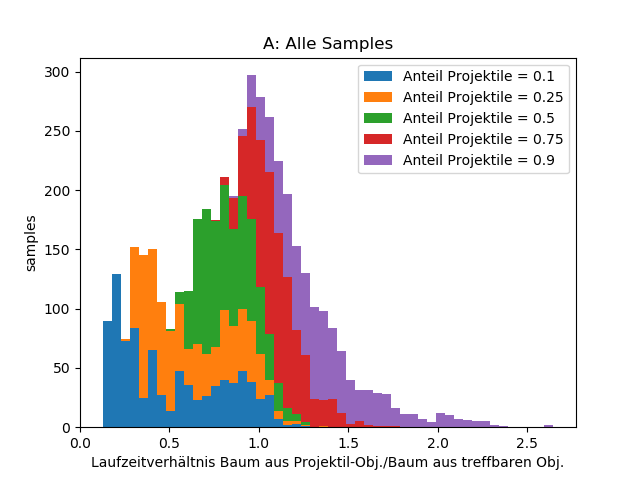
\includegraphics[width=1\textwidth]{./res/boxsortChoice-shotgun-A.png}
		
		\label{fig:boxsortChoice-shotgun-A}
	\end{subfigure}
~
	\begin{subfigure}[t]{0.55\textwidth}
		\centering
		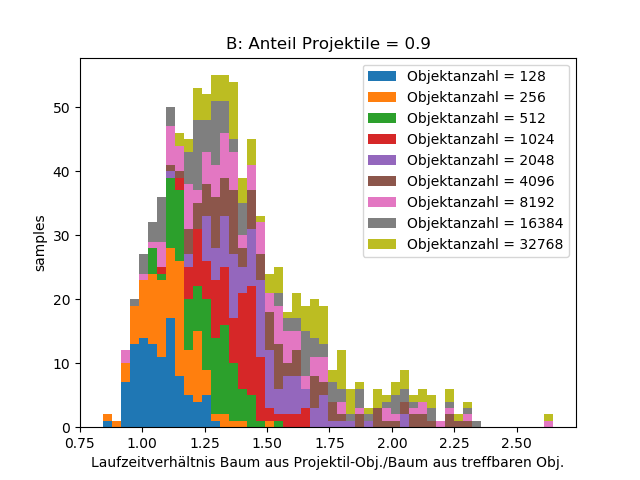
\includegraphics[width=1\textwidth]{./res/boxsortChoice-shotgun-B.png}

		\label{fig:boxsortChoice-shotgun-B}
	\end{subfigure}
~
	\begin{subfigure}[t]{0.55\textwidth}
		\centering
		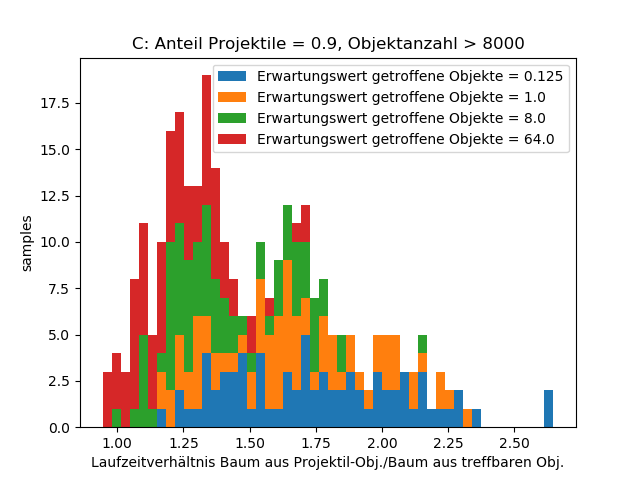
\includegraphics[width=1\textwidth]{./res/boxsortChoice-shotgun-C.png}

		\label{fig:boxsortChoice-shotgun-C}
	\end{subfigure}
~
	\begin{subfigure}[t]{0.55\textwidth}
		\centering
		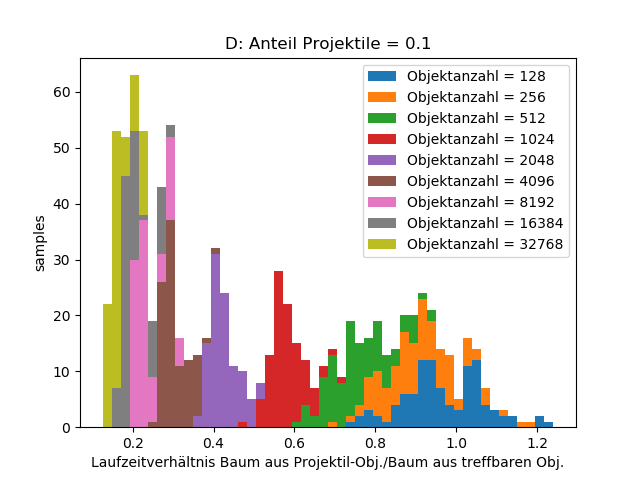
\includegraphics[width=1\textwidth]{./res/boxsortChoice-shotgun-D.png}

		\label{fig:boxsortChoice-shotgun-D}
	\end{subfigure}
~
	\begin{subfigure}[t]{0.55\textwidth}
		\centering
		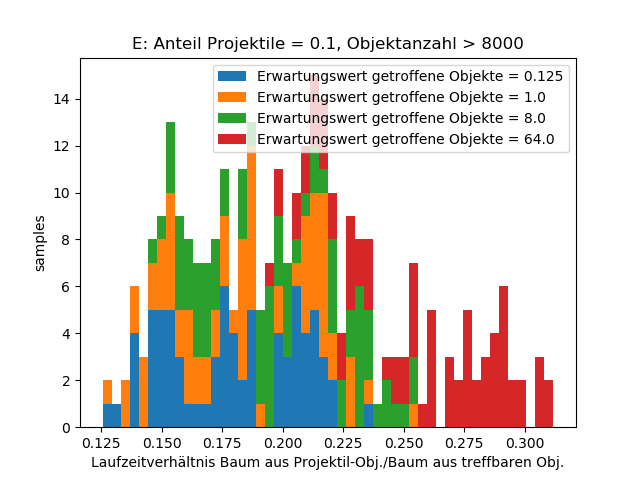
\includegraphics[width=1\textwidth]{./res/boxsortChoice-shotgun-E.png}

		\label{fig:boxsortChoice-shotgun-E}
	\end{subfigure}


	\caption{Untersuchung der Auswirkungen verschiedener Parameter auf das Verhältnis der Laufzeiten des Box Sort Algorithmus im Shotgun-Szenario. Dargestellt sind Histogramme mit nach einem Parameter getrennten Samples, mit den jeweiligen Balken aufeinandergestapelt.}
	\label{fig:boxsortChoice-shotgun}
\end{figure*}



\begin{figure*}

	\begin{subfigure}[t]{0.55\textwidth}
		\centering
		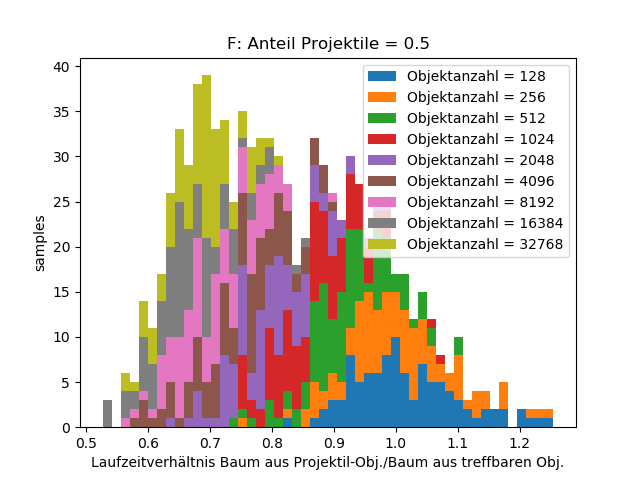
\includegraphics[width=1\textwidth]{./res/boxsortChoice-shotgun-F.png}
		
		\label{fig:boxsortChoice-shotgun-F}
	\end{subfigure}
~
	\begin{subfigure}[t]{0.55\textwidth}
		\centering
		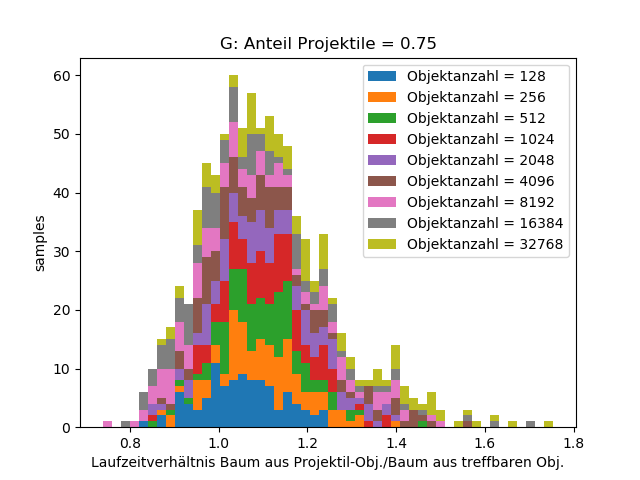
\includegraphics[width=1\textwidth]{./res/boxsortChoice-shotgun-G.png}

		\label{fig:boxsortChoice-shotgun-G}
	\end{subfigure}

	\caption{Untersuchung der Auswirkungen verschiedener Parameter auf das Verhältnis der Laufzeiten des Box Sort Algorithmus im Shotgun-Szenario. Hier werden konkret andere Werte für den Anteil an Projektil-Objekten untersucht. Dargestellt sind Histogramme mit nach einem Parameter getrennten Samples, mit den jeweiligen Balken aufeinandergestapelt.}
	\label{fig:boxsortChoice-shotgun2}
\end{figure*}

Die Objekte sind in der Praxis jedoch nicht immer gleich verteilt. Als nächstes wird deshalb das Szenario \glqq Shotgun\grqq ~betrachtet. In Abb.~\ref{fig:boxsortChoice-shotgun} A ist zu sehen, dass wie bei der Gleichverteilung meist die kleinere Menge verwendet werden sollte. Die Menge der Samples, wo dies nicht zutrifft ist jedoch größer als bei der Gleichverteilung. Abb.~\ref{fig:boxsortChoice-uniform} B zeigt nur die Samples, wo der Projektilanteil 90\% beträgt. Zu erkennen ist, dass eine höhere Objektanzahl die Abweichung verstärkt. In Abb.~\ref{fig:boxsortChoice-uniform} D sieht man, dass bei umgedrehtem Klassenanteil diese Abweichung noch extremer wird. Dies lässt eine Tendenz vermuten, die in Abb.~\ref{fig:boxsortChoice-uniform2} bestätigt wird. Dort sieht man, dass erst bei einem Projektilantil von 75\% (nicht aber bei 50\%) die Objektanzahl kaum mehr einen Einfluss hat.\\
Nun wird noch der Einfluss des Erwartungswerts getroffener Objekte untersucht, wenn die Objektzahl hoch ist. In Abb.~\ref{fig:boxsortChoice-shotgun} C ist zu erkennen, dass bei einem Projektilanteil von 90\% ein geringerer Erwartungswert das Verhältnis nach oben beeinflusst und eine erheblich größere Streuung der Samples verursacht. In Abb.  ~\ref{fig:boxsortChoice-shotgun} E ist erkennbar, dass bei umgekehrtem Klassenanteil ebenfalls ein höherer Erwartungswert getroffener Objekte das Verhältnis in Richtung 1 bewegt.\\


\begin{figure*}
	\begin{subfigure}[t]{0.55\textwidth}
		\centering
		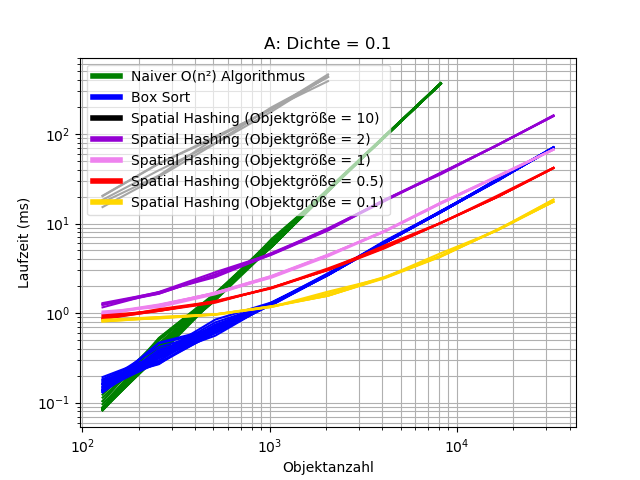
\includegraphics[width=1\textwidth]{./res/symmetricComparison-A.png}
		
		\label{fig:symmetricComparison-A}
	\end{subfigure}
~
	\begin{subfigure}[t]{0.55\textwidth}
		\centering
		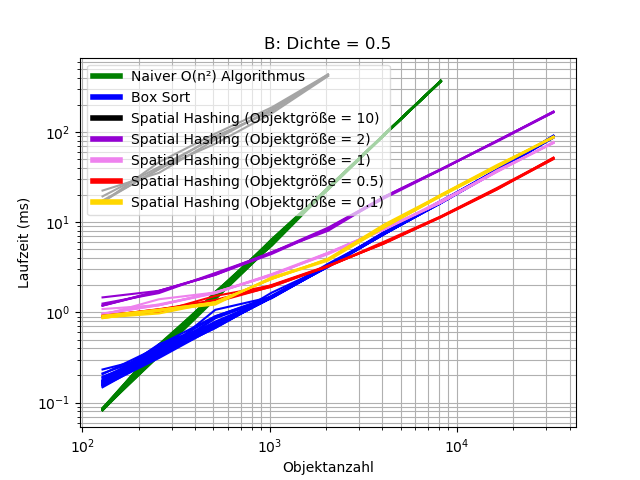
\includegraphics[width=1\textwidth]{./res/symmetricComparison-B.png}

		\label{fig:symmetricComparison-B}
	\end{subfigure}
~
	\begin{subfigure}[t]{0.55\textwidth}
		\centering
		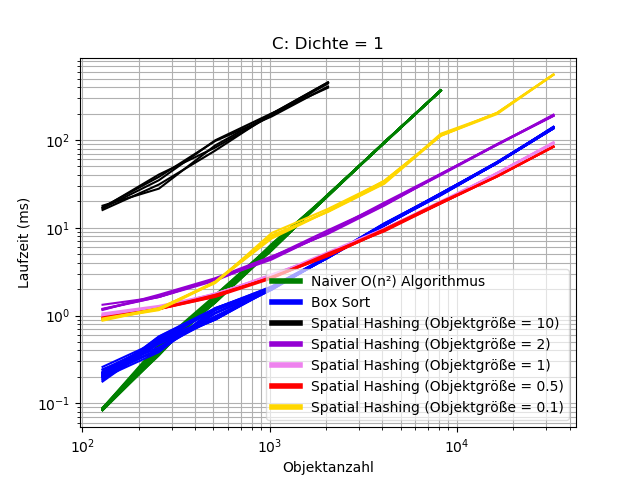
\includegraphics[width=1\textwidth]{./res/symmetricComparison-C.png}

		\label{fig:symmetricComparison-C}
	\end{subfigure}
~
	\begin{subfigure}[t]{0.55\textwidth}
		\centering
		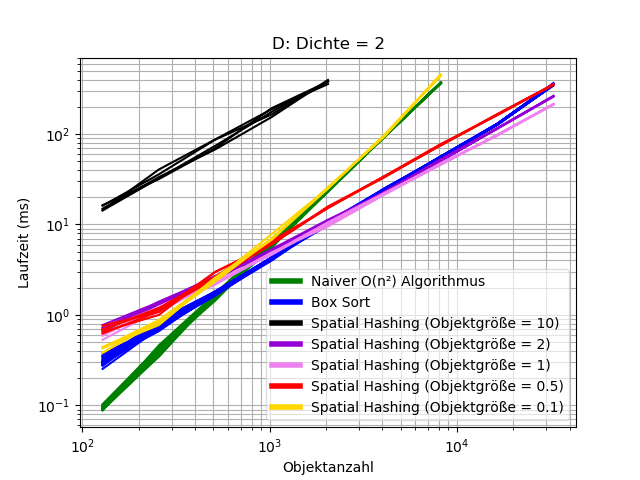
\includegraphics[width=1\textwidth]{./res/symmetricComparison-D.png}

		\label{fig:symmetricComparison-D}
	\end{subfigure}
~
	\begin{subfigure}[t]{0.55\textwidth}
		\centering
		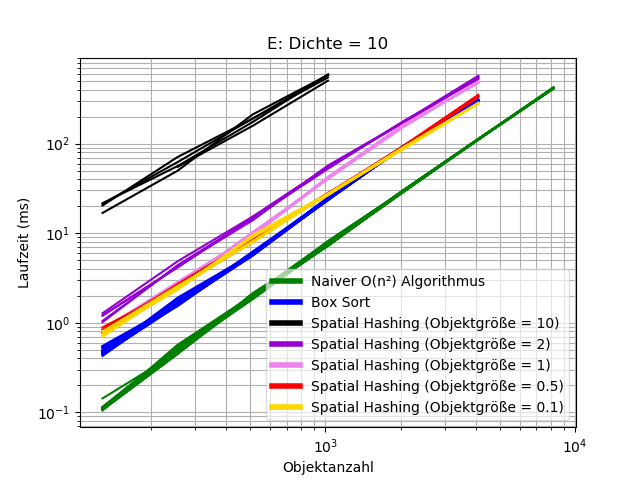
\includegraphics[width=1\textwidth]{./res/symmetricComparison-E.png}

		\label{fig:symmetricComparison-E}
	\end{subfigure}
~
	\begin{subfigure}[t]{0.55\textwidth}
		\centering
		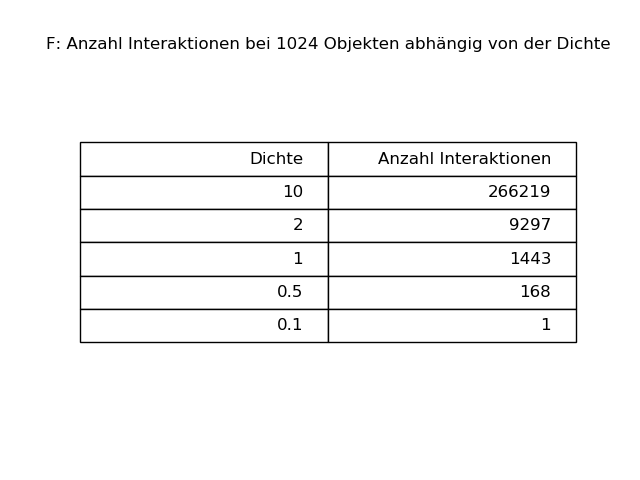
\includegraphics[width=1\textwidth]{./res/symmetricComparison-F.png}

		\label{fig:symmetricComparison-F}
	\end{subfigure}

	\caption{Alle Benchmark-Daten für das gleich verteilte Szenario bei symmetrischen Interaktionen, aufgeteilt nach Dichte. Die Tabelle F zeigt die Anzahl Interaktionen bei jeweils einer Beispiel-Aufgabenstellung mit 1024 Objekten und verschiedenen Dichten.}
	\label{fig:symmetricComparison}
\end{figure*}

In Abb.~\ref{fig:symmetricComparison} wird nun die Performance von allen Algorithmen verglichen, zunächst im Fall symmetrischer Interaktionen. Das einzige hierbei betrachtete Szenario ist eine Gleichverteilung der Objekte. Nahe liegt die Annahme, dass die Größe von Objekten (in $\mathcal{S}$) keinen Einfluss auf den naiven Algorithmus und Box Sort haben, da diese nur mit relativen Größen und Vergleichen arbeiten. Während der Auswertung wurde jedoch festgestellt, dass dies nicht der Fall war. Vergleichsoperationen und Rechnungen in $\mathcal{S}$ verwendeten Branches, die von der Größe der Unterschiede zwischen den Operanden abhängen. Um diese Variable zu eliminieren wurden Techniken des Branchless Programming eingesetzt. Dies hat sich zudem als Optimierung um ca. 0-50\% je nach Umständen herausgestellt und wurde somit beibehalten. Alle abgebildeten Daten (auch die weiter oben) beinhalten diese Änderung.\\
Die Graphen von Box Sort und dem naiven Algorithmus behandeln die Samples mit verschiedenen Objektgrößen identisch. Sie sind als mehrere Linien im Diagramm eingetragen, genau wie zu jedem Parametersatz die 4 Samples, die sich nur im Seed für die Generierung der Aufgabenstellung unterscheiden. Dargestellt ist die Laufzeit in Abhängigkeit von der Objektanzahl. Die Samples, immer um Faktor 2 auseinander, werden linear interpoliert zu einem Graph verbunden. Zu sehen ist, dass Spatial Hashing empfindlich auf die Größe der Objekte relativ zur Größe der Chunks reagiert. Sind die Objekte z.B. durchschnittlich 10-mal größer als Chunks, ist die Performance besonders schlecht. Dies ist intuitiv verständlich, da sich jedes Objekt bei durchschnittlich 1000 Chunks anmelden und dort nach Interaktionspartnern suchen muss. Der naive Algorithmus zeigt wie zu erwarten kaum eine Abhängigkeit von der Dichte und hat die kleinste Konstante, was vor allem bei kleiner Menge and Objekten die beste Performance liefert. Box Sort hat eine konsistent gute Performance, sodass er nur bei extrem hoher Dichte oder geringer Menge an Objekten eine längere Laufzeit als der naive Algorithmus benötigt. Spatial Hashing hat in vielen Situationen vor allem bei größeren Objektmengen eine noch bessere Performance, ist aber weniger flexibel bei der Objektgröße. Neben dem offensichtlichen Problem bei großen Objekten ist auch eine zu kleine Objektgröße bei gegebener Dichte für Spatial Hashing nachteilig, da sich dann mehr Objekte innerhalb eines Chunks befinden und innerhalb eines Chunks der naive Algorithmus verwendet wird. Je nach Dichte ist eine andere Objektgröße ideal. Bei geringer Dichte überwiegt der Laufzeitanteil der Anmeldung in (und damit Erstellung von) Chunks, sodass dort möglichst kleine Objekte in weniger Chunks enthalten sind. Wenn die Dichte höher wird, nähert sich die ideale Objektgröße an die Chunkgröße an. Für extreme Dichten ist Spatial Hashing genau wie Box Sort ungeeignet.\\


\begin{figure*}
	\begin{subfigure}[t]{0.55\textwidth}
		\centering
		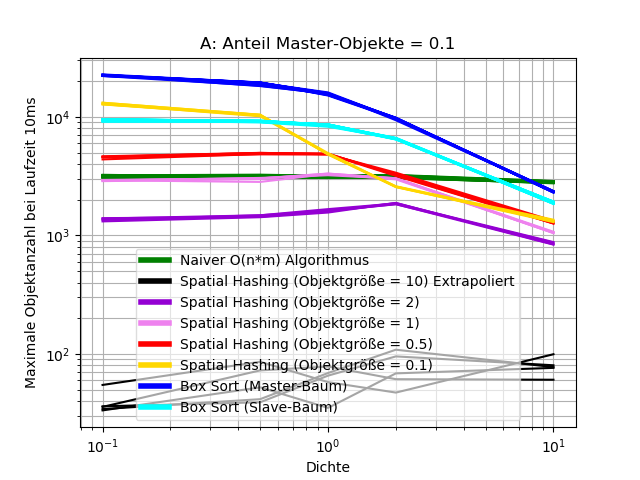
\includegraphics[width=1\textwidth]{./res/asymComparison-A.png}
		
		\label{fig:asymComparison-A}
	\end{subfigure}
~
	\begin{subfigure}[t]{0.55\textwidth}
		\centering
		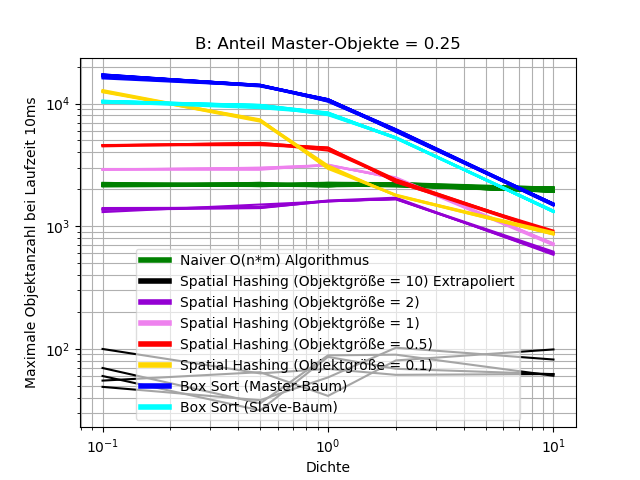
\includegraphics[width=1\textwidth]{./res/asymComparison-B.png}

		\label{fig:asymComparison-B}
	\end{subfigure}
~
	\begin{subfigure}[t]{0.55\textwidth}
		\centering
		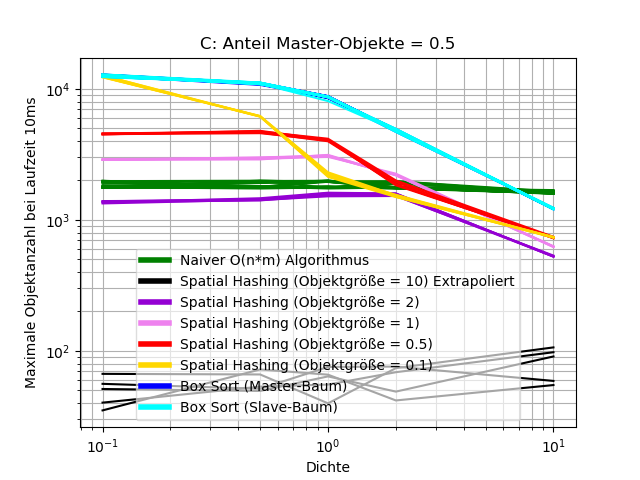
\includegraphics[width=1\textwidth]{./res/asymComparison-C.png}

		\label{fig:asymComparison-C}
	\end{subfigure}
~
	\begin{subfigure}[t]{0.55\textwidth}
		\centering
		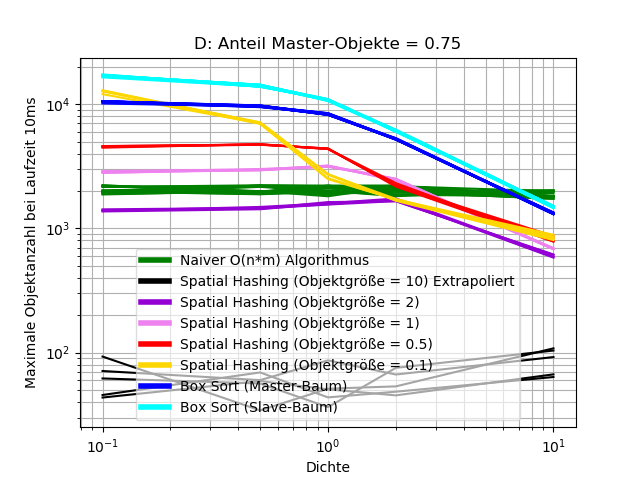
\includegraphics[width=1\textwidth]{./res/asymComparison-D.png}

		\label{fig:asymComparison-D}
	\end{subfigure}
~
	\begin{subfigure}[t]{0.55\textwidth}
		\centering
		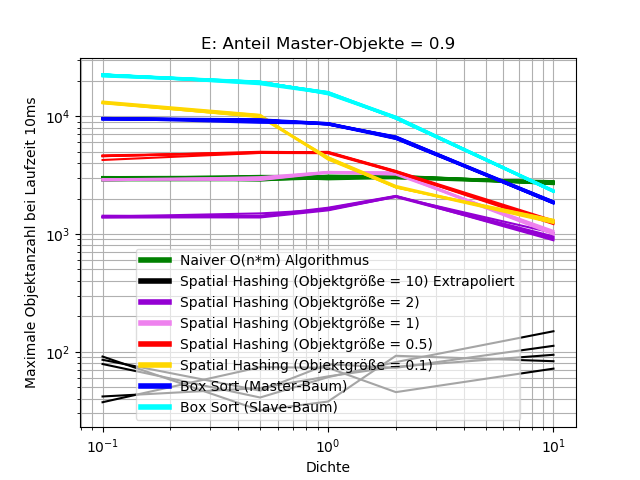
\includegraphics[width=1\textwidth]{./res/asymComparison-E.png}

		\label{fig:asymComparison-E}
	\end{subfigure}
~
	\begin{subfigure}[t]{0.55\textwidth}
		\centering
		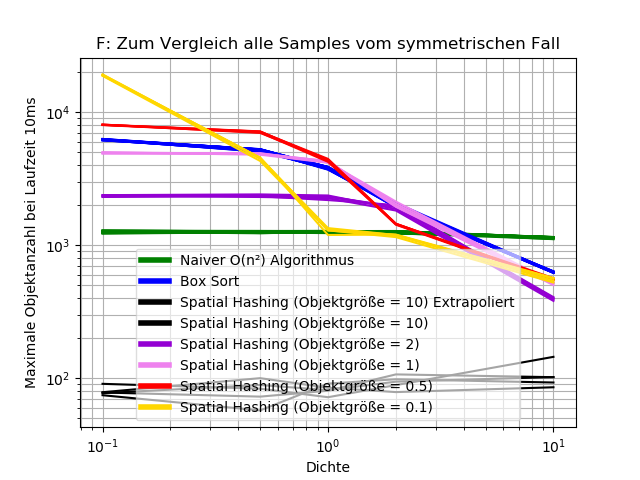
\includegraphics[width=1\textwidth]{./res/asymComparison-F.png}

		\label{fig:asymComparison-F}
	\end{subfigure}

	\caption{Alle Benchmark-Daten für das gleichverteilte Szenario bei asymmetrischen Interaktionen, aufgeteilt nach dem Anteil der Objekte, die der Master-Klasse angehören. Zum Vergleich wurde die gleiche Art Graph aus allen Daten bei symmetrischen Interaktionen erzeugt.}
	\label{fig:asymComparison}
\end{figure*}

Die Szanarien mit asymmetrischen Interaktionen haben einen Parameter mehr, sodass eine kompaktere Version der Graphen benötigt wird, um effizient alle Daten darzustellen. Dazu wird eine Annahme über den Verwendungszweck gemacht, der für die meisten Videospiele und viele Echtzeit-Simulationen zutrifft: Es steht eine bestimmte Zeit zur Verfügung, in der alle Berechnungen abgeschlossen sein müssen. Hier wurde also untersucht, für wie viele Objekte in 10ms alle Interaktionen berechnet werden können. Der Zeitrahmen ist dabei weniger strikt wie z.B. in professionellen Counter-Strike Matches aber strikter als in Videospielen wie Minecraft. 10ms erscheint eher im strikten Bereich, aber es muss auch beachtet werden, dass die Ausführung dieses Algorithmus nicht das Einzige ist, was in einer Simulation Rechenzeit benötigt. Die maximale Objektanzahl wurde durch lineare Interpolation der getesteten Samples ermittelt. Für Fälle, wo die Anzahl außerhalb des getesteten Bereichs liegt (größer 32768 oder kleiner 128), wird stattdessen extrapoliert. Wenn ein Großteil der Samples außerhalb liegt, ist in der Legende \glqq Extrapoliert\grqq ~vermerkt.\\
Abb.~\ref{fig:asymComparison} zeigt das gleichverteilte Szenario, unterteilt nach dem Anteil der Objekte, die der Master-Klasse angehören. Zum Vergleich wurden alle Daten des symmetrischen Falls des gleichverteilten Szenarios auf die gleiche Art ausgewertet (Abb.~\ref{fig:asymComparison} F). Die Dichte ist nun auf der x-Achse. Im Vergleich zum symmetrischen Fall ist die erreichte Anzahl beim naiven Algorithmus höher, da nicht alle Objekte mit allen anderen getestet werden müssen, sondern nur Paare mit jeweils einem Objekt aus einer Klasse ($\mathcal{O}(|\obj_M|*|\obj_S|)$). Dies ist besonders deutlich bei einer 10\% - 90\% Aufteilung. Box Sort hat bei asymmetrischen Interaktionen ebenfalls einen Vorteil, der noch stärker ausgeprägt ist. Dies stammt von dem Problem bei symmetrischen Interaktionen, dass aufgrund der Funktionsweise alle Interaktionen in beide Richtungen gefunden werden und die eine Richtung herausgefiltert werden muss, die Effizienz ist dort also nur 50\%. Dies ist bei asymmetrischen Interaktionen nicht der Fall. Bei Spatial Hashing ist die Laufzeit zum Anmelden in und Anlegen von Chunks bei asymmetrischen Interaktionen nicht positiv beeinflusst. Deshalb ist selbst unter ansonsten idealen Umständen (geringe Dichte) die Performance gegenüber Box Sort nicht mehr überlegen.\\
Abb.~\ref{fig:asymComparison} A und Abb.~\ref{fig:asymComparison} E bzw. Abb.~\ref{fig:asymComparison} B und Abb.~\ref{fig:asymComparison} D weisen starke Ähnlichkeiten zueinander auf. Dies ist nicht verwunderlich, da sie nur dem Tausch der Master-Objekte mit Slave-Objekten entsprechen. Die Graphen für Box Sort mit Baum aus Master-Objekten und Slave-Objekten sind entsprechend vertauscht. Eventuelle Unterschiede zwischen den jeweiligen Teilabbildungen könnten auf verschiedene Ergebnisse der Pseudozufälligen Aufgabengenerierung zurückzuführen sein. Geringfügige Unterschiede der Trends der Graphen könnten mit Caching in der CPU zusammenhängen, denn es werden zuerst alle Master-Objekte generiert, dann die Slave-Objekte, der Cache-Inhalt ist also beim Start der Algorithmen nicht ebenfalls vertauscht.\\
Diese Symmetrie ist beim Shotgun-Szenario nicht vorhanden, da dort die beiden Mengen nicht die gleiche statistische Verteilung aufweisen. Abb.~\ref{fig:shotgunComparison} zeigt die Daten dieses Szenarios. Die x-Achse ist nun der Erwartungswert der Anzahl treffbarer Objekte in dem Bereich, wo Projektil-Objekte erzeugt werden. Es wurden 4 Werte getestet, jeweils um den Faktor 8 verschieden. Zu sehen ist eine viel höhere Abweichung der Samples auch bei Werten, die im Gleichverteilungs-Szenario keine solche aufweisen. Diese stammen wahrscheinlich daher, dass die konkret generierte Aufgabenstellung eine hohe Abweichung der Anzahl der Interaktionen aufweist. Dies ist wegen dem kompakten Bereich der Fall, worin alle Projektil-Objekte generiert werden. Nur eine geringe Anzahl treffbarer Objekte ist darin enthalten, was statistisch zu einer hohen Standardabweichung relativ zum Erwartungwert führt. Die Objekte in dem Bereich interagieren dann mit einem großen Teil aller Projektil-Objekte.\\
Allgemein ist beim Shotgun-Szenario Box Sort wieder überlegen. Den Baum aus Projektil-Objekten aufzubauen hat hier einen Vorteil: die meisten treffbaren Objekte können wegen der Kompaktheit des Projektil-Erzeugungsbereichs schon beim root-Knoten ausgeschlossen werden.\\

\begin{figure*}
	\begin{subfigure}[t]{0.55\textwidth}
		\centering
		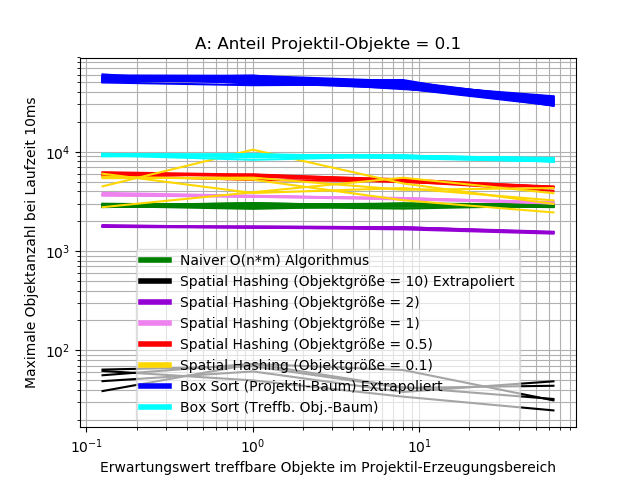
\includegraphics[width=1\textwidth]{./res/shotgunComparison-A.png}
		
		\label{fig:shotgunComparison-A}
	\end{subfigure}
~
	\begin{subfigure}[t]{0.55\textwidth}
		\centering
		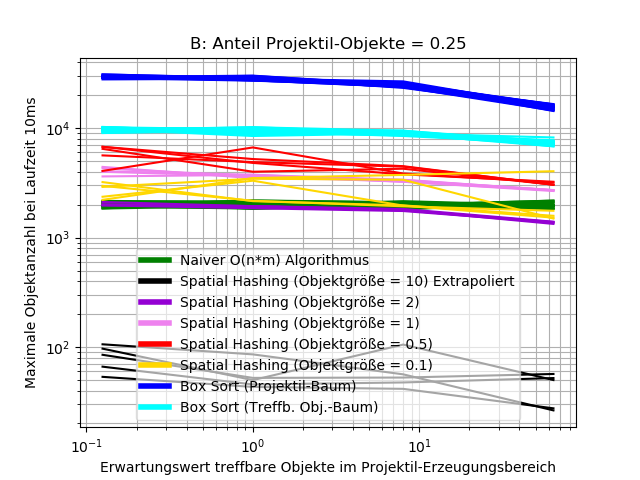
\includegraphics[width=1\textwidth]{./res/shotgunComparison-B.png}

		\label{fig:shotgunComparison-B}
	\end{subfigure}
~
	\begin{subfigure}[t]{0.55\textwidth}
		\centering
		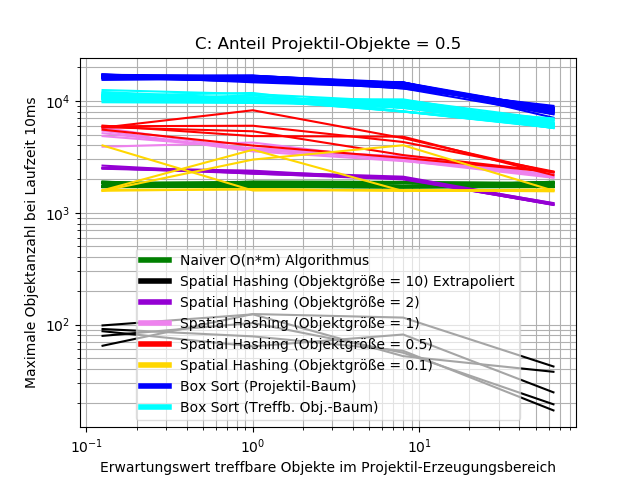
\includegraphics[width=1\textwidth]{./res/shotgunComparison-C.png}

		\label{fig:shotgunComparison-C}
	\end{subfigure}
~
	\begin{subfigure}[t]{0.55\textwidth}
		\centering
		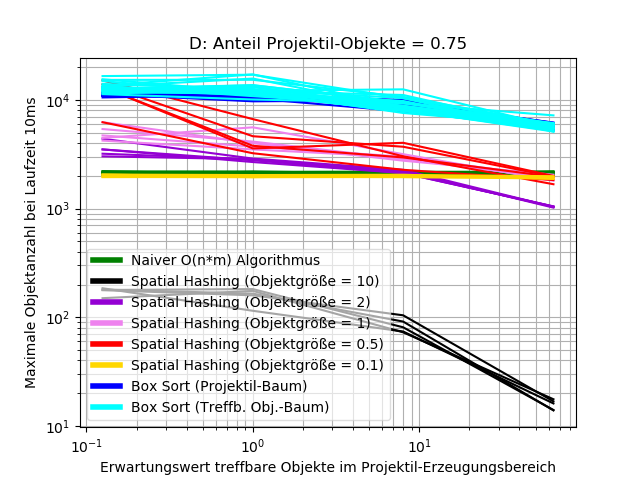
\includegraphics[width=1\textwidth]{./res/shotgunComparison-D.png}

		\label{fig:shotgunComparison-D}
	\end{subfigure}
~
	\begin{subfigure}[t]{0.55\textwidth}
		\centering
		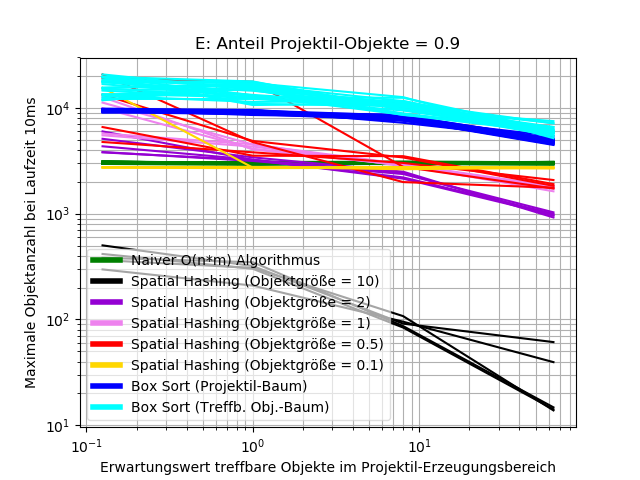
\includegraphics[width=1\textwidth]{./res/shotgunComparison-E.png}

		\label{fig:shotgunComparison-E}
	\end{subfigure}

	\caption{Alle Benchmark-Daten für das Shotgun-Szenario, aufgeteilt nach dem Anteil der Objekte, die der Projektil-Klasse angehören.}
	\label{fig:shotgunComparison}
\end{figure*}

\subsection{Fazit und Ausblick}
Als Fazit kann man sagen, dass beide Algorithmen für die Praxis tauglich sind, mit Boxsort als robuster Mittelweg und  Spatial Hashing (mit richtiger Konfiguration) für bessere Performance bei bestimmten Anwendungen. Games sollten also diese oder andere ähnlich performante Verfahren zur Kollisionsvorfilterung verwenden. Dies ist bei vielen aktuell am Markt befindlichen Spielen leider nicht der Fall, was bei einer hohen Objektanzahl selbst ohne Kollisionen zu einer schlechten Performance führt. Dies ist meist bei Indie-Games der Fall, auch weil dort typischerweise weniger Limits existieren, die den Spieler davon abhalten, ein solches Problem erst zu erzeugen. Hier wird vermutet, dass einer der Gründe für eine fehlende Implementierung solcher besseren Algorithmen ist, dass von Entwicklern meist nur mit dem Durchschnittsspieler gerechnet wird, für den die Probleme meist nicht auftreten. Ein weiterer könnte sein, dass sich der Aufwand monetär nicht lohnt, da man als Spieler die Probleme meist erst dann hat, wenn man bereits das Spiel und eventuelle Erweiterungen gekauft hat.\\

Da dieses Projekt aus privatem Interesse entstanden ist, wäre es nicht unrealistisch anzunehmen, dass an den Vorfilterungsalgorithmen in Zukunft weiter gearbeitet wird. Beim Spatial Hashing ist ein für die Praxis relevantes Problem, dass aktuell die Größe von Chunks an die Größe der Einheitslänge in $\mathcal{S}$ gebunden ist. Man könnte einen Parameter einfügen, der sie um genzzahlige Faktoren größer (aber nicht kleiner) werden ließe, ohne die durch die Bindung gewonnene Performance stark zu beeinflussen. Der Wertebereich der Eingabe der Hashfunktion wäre dann nicht beeinflusst. Es könnte außerdem untersucht werden, warum die Performance beim Spatial Hashing bei geringer Objektanzahl so schlecht ist. Bei Box Sort könnte man u.a. die Medianfindung analysieren, um die Performance eventuell zu verbessern. Auch eine Implementierung des Baums, die stärker das Cache-Verhalten ausnutzt, wäre denkbar.\\
Für hohe absolute Geschwindigkeiten könnten AABBs mit Geschwindigkeit implementiert werden, so könnte man eventuell auch einen ganzen Knoten im Baum von Boxsort mit einer Geschwindigkeit versehen. Eine Art hierarchische Baumstruktur könnte auch bei der Kollision von 2 konkreten Objekten hilfreich sein, um Teile des Objekts mit AABBs zu versehen und sie so verfrüht von der rechenintensiven Kollisionsberechnung auszuschließen.\\

//TODO 2.6 rework
